%!TEX root = paper.tex

\newcommand{\videoDataVsStorageFigure}{
\begin{figure}[h]
  \centering
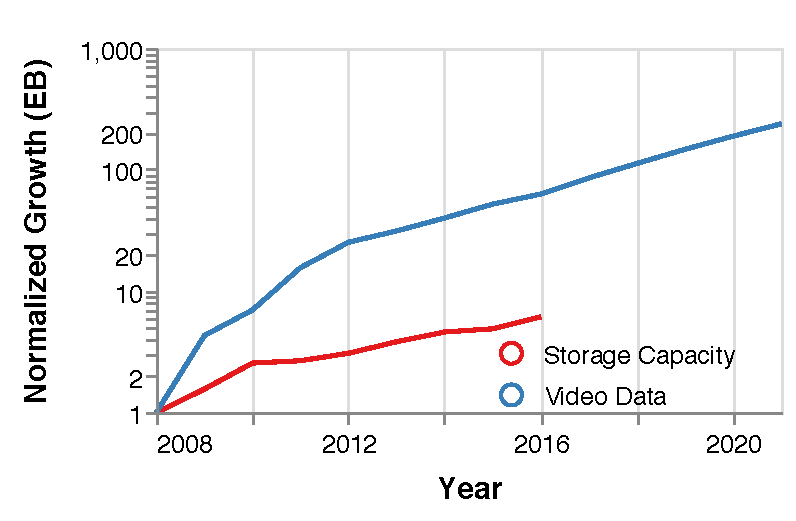
\includegraphics[width=\linewidth]{vignette-figs/storage-video-growth.pdf}
  \caption{Normalized growth of total storage produced and video data captured since 2008~\cite{cisco2016zettabyte,fontana2018storage}. Video data is outgrowing  storage capacity, taxing storage system capacity.}
  \label{plot:video-data-vs-storage}
\end{figure}
}

\newcommand{\tileVsSizeFigure}{
\begin{figure}
  \centering
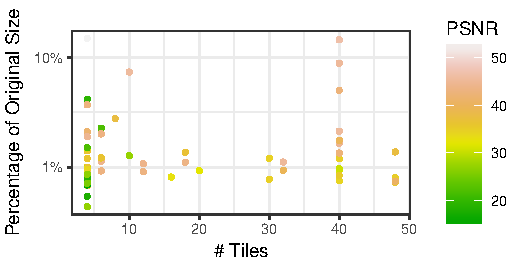
\includegraphics[width=.8\linewidth]{vignette-figs/tileSizeQuality2.pdf}
  \caption{Compression ratio and PSNR at the optimal number of tiles for each video. The optimal number of tiles is video-dependent, not correlated with quality or compression ratio.}
  \label{plot:tile-vs-size}
\end{figure}
}

\newcommand{\computeTable}{
\begin{table}[h]
\centering
\caption{Mean processing time per video, evaluated over all videos in our datasets.}
\label{table:compute}

\begin{tabular}{lrcrc} \toprule
   & \multicolumn{2}{c}{Exhaustive} & \multicolumn{2}{c}{Heuristic }\\
    \cmidrule(lr){2-3}\cmidrule(lr){4-5}
  Task                       & Time (s) & \%   & Time (s) & \% \\ \midrule
  Generate saliency map      & 1633     & 49\% &  1633     & 95\%   \\
  Compute tile configuration & 1696     & 50\phantom{\%} &  59      & 4\phantom{\%}   \\
  Saliency-based transcode   & 21       & \phantom{0}1\phantom{\%}  &  21      & \phantom{0}1\phantom{\%}   \\ \midrule
  Total                      & 3350     &      &  1713     & \\ \bottomrule
\end{tabular}

\end{table}

}

\newcommand{\userStudyFigure}{

\begin{figure*}
  \centering
  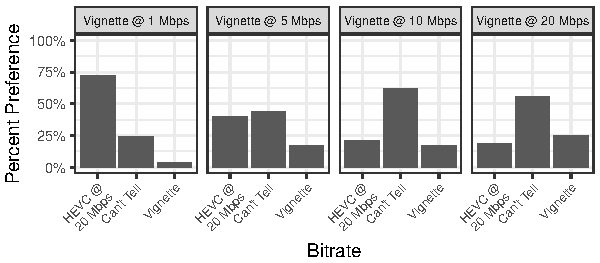
\includegraphics[width=.7\linewidth]{vignette-figs/user-study.pdf}
  \caption{Results of perceived quality preference user study, averaged across participants and videos by bitrate. Participants either preferred \name or perceived no difference between 20 Mbps \hevc videos and \name videos at 5--20 Mbps.}
  \label{plot:user-study}
\end{figure*}
}
\newcommand{\failureModeFigure}{

\begin{figure}[h]
  \centering
  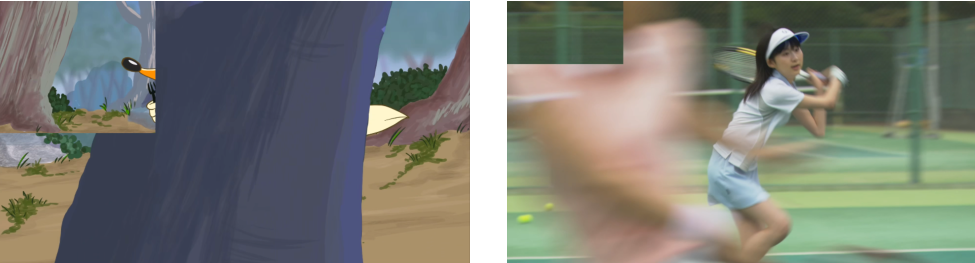
\includegraphics[width=\linewidth]{vignette-figs/tile-failure.pdf}
  \caption{Two instances of failure from tiling (top-left tile) during fast-motion sequences.}
  \label{fig:vignette-failures}
\end{figure}
}


\newcommand{\vbenchScoreFigure}{
\begin{figure}[h]
  \centering
  \includegraphics[width=\linewidth]{vignette-figs/vbench-scores.pdf}
  \caption{\texttt{vbench} scores comparing \nameCompress to their reference. \todo{fake data}}
  \label{plot:vbench}
\end{figure}
}

\newcommand{\saliencyTilesOverviewFigure}{
\begin{figure}
  \centering
  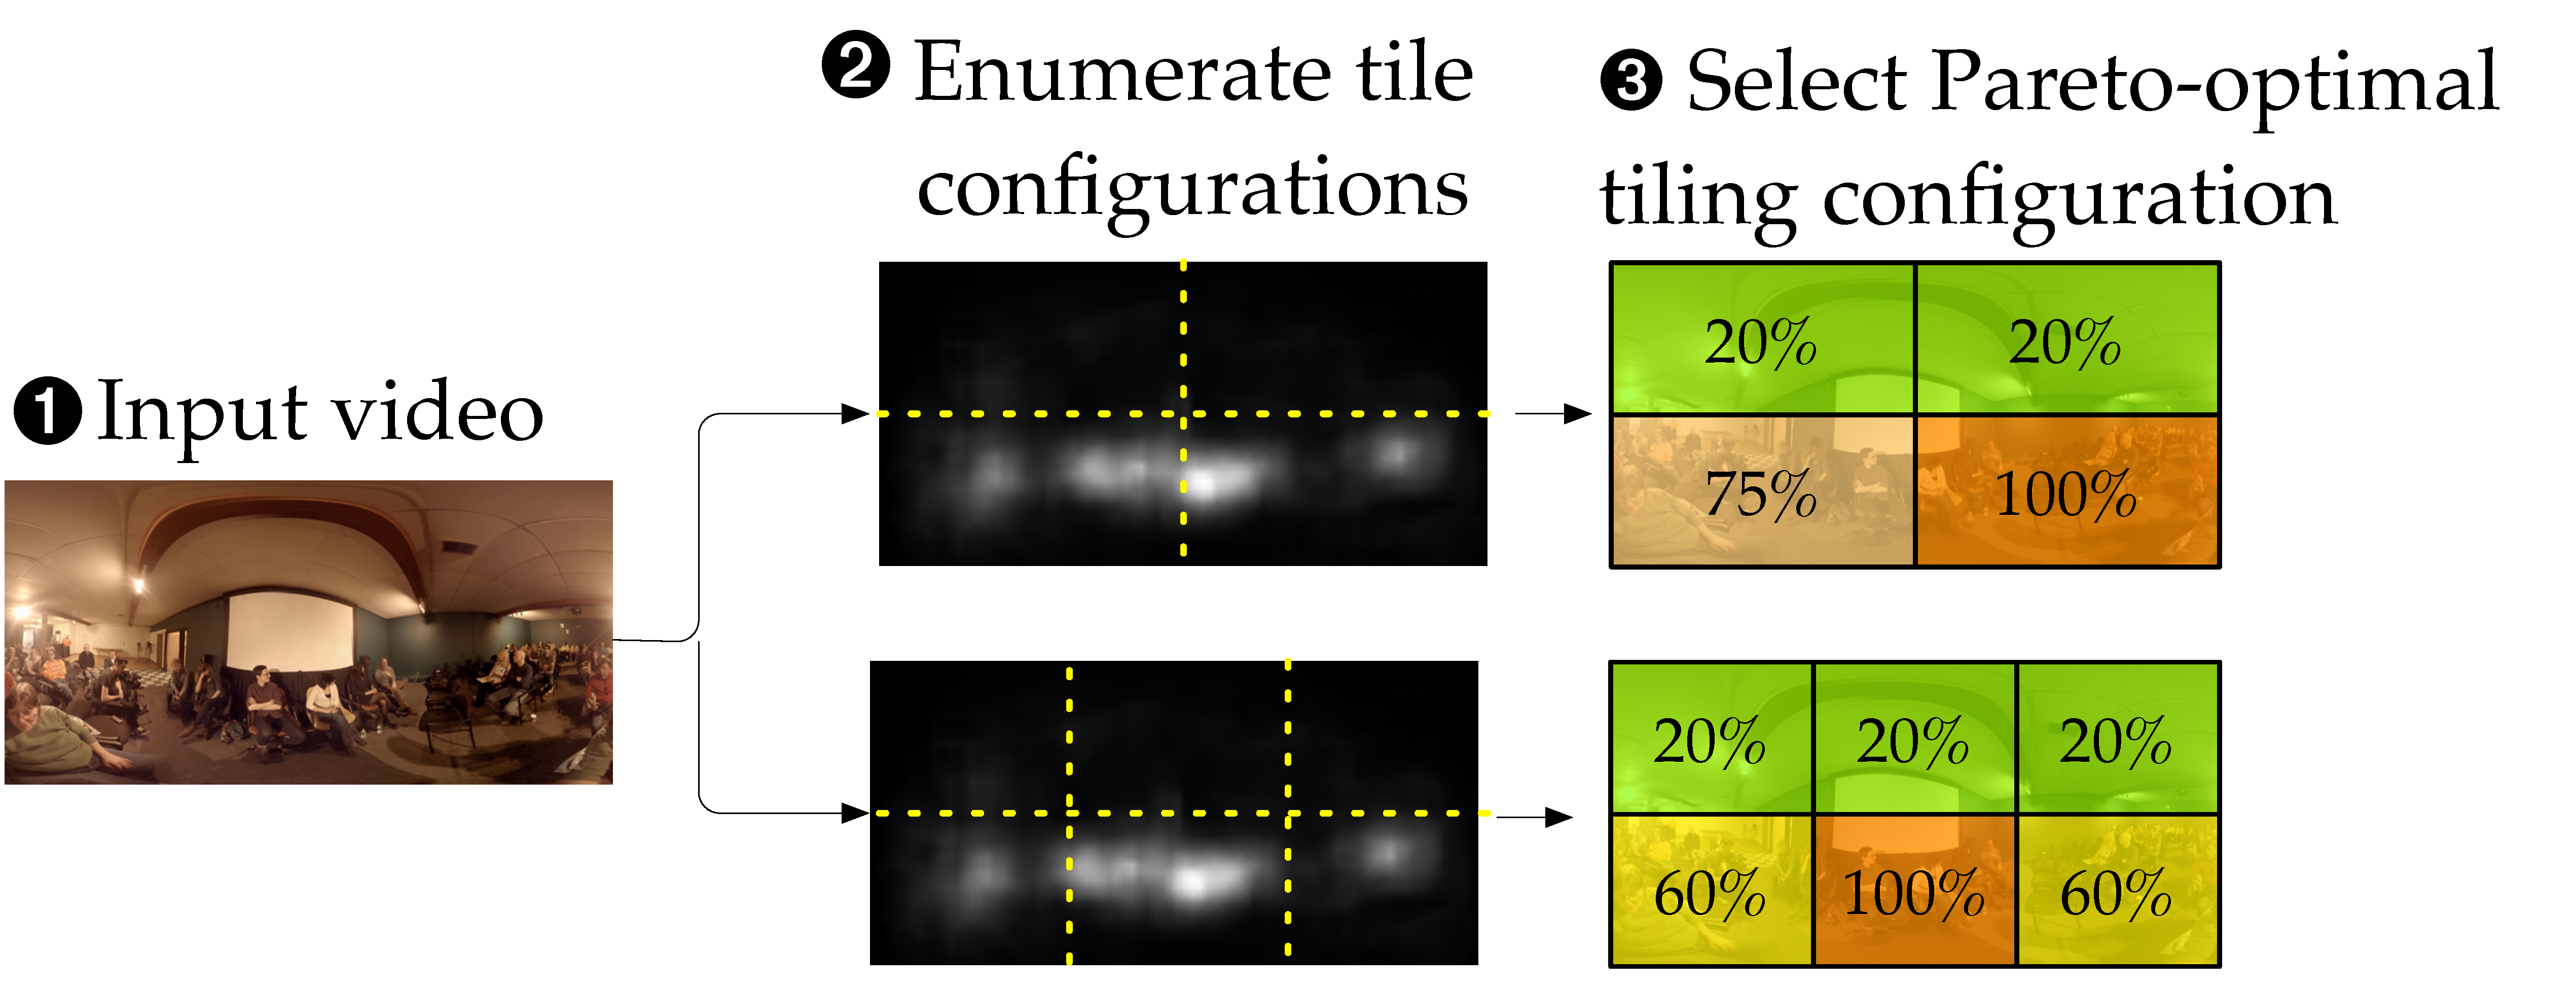
\includegraphics[width=\textwidth]{vignette-figs/tiled-bitrate}
  \caption{Overview of \nameCompress algorithm.}
  \label{fig:saliency-tiles-overview}
\end{figure}
}

\newcommand{\architectureOverviewFigure}{
\begin{figure}
  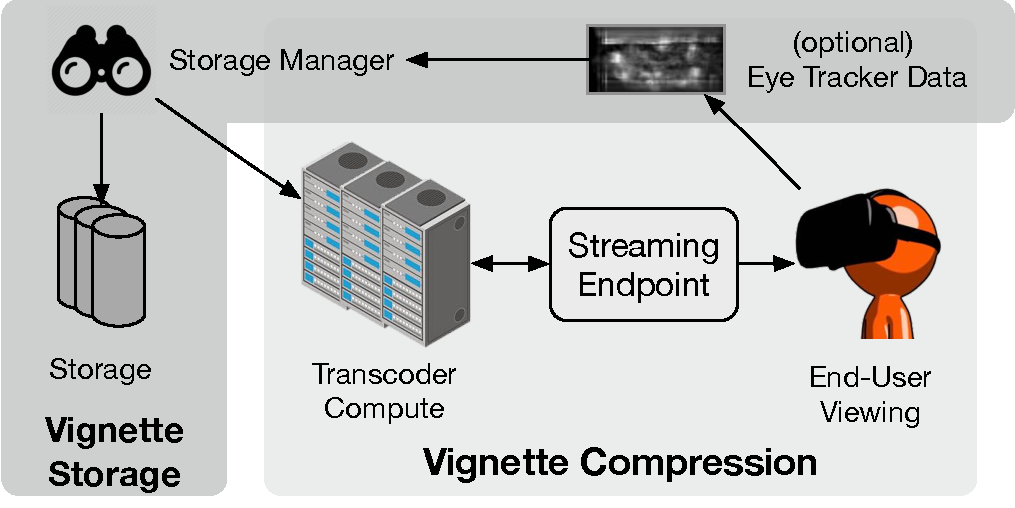
\includegraphics[width=\textwidth]{vignette-figs/high-level-architecture}
  \caption{\name provides two features: \nameCompress, a perceptual compression algorithm, and \nameStore, a storage manager for perceptually compressed videos.
  Integrating perceptual information with the storage manager reduces network bandwidth and storage costs.}
  \label{fig:high-level-architecture}
\end{figure}


}

\newcommand{\exampleVidSaliencyFigure}{

\begin{figure}
  \centering
  % \begin{subfigure}{.32\textwidth}
  %   \centering
  %   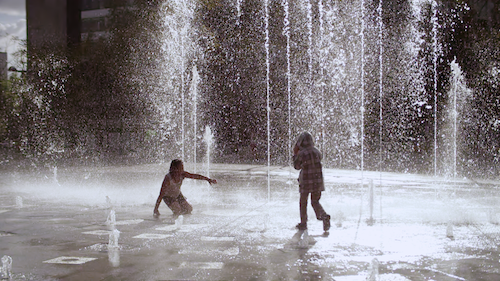
\includegraphics[width=.9\linewidth]{vignette-figs/elfuente_in.png}
  %   \caption{Input video frame from Netflix dataset~\cite{netflix2016data}.}
  %   \label{subfig:og-stil}
  % \end{subfigure}%
  % \begin{subfigure}{.32\textwidth}
  %   \centering
  %   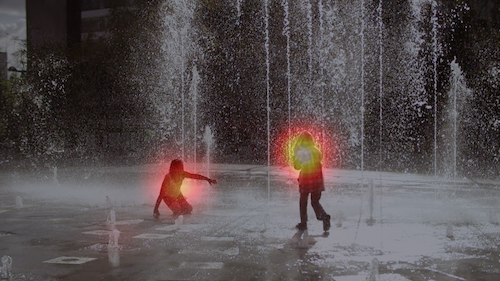
\includegraphics[width=.9\linewidth]{vignette-figs/elfuente_sal.png}
  %   \caption{Saliency map, produced by MLNet~\cite{mlnet2016}, overlaid on input.}
  %   \label{subfig:sal-still}
  % \end{subfigure}%
  % \begin{subfigure}{.32\textwidth}
  %   \centering
  %   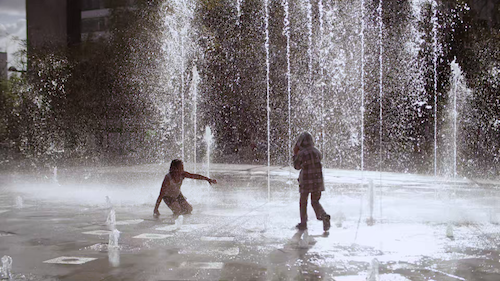
\includegraphics[width=.9\linewidth]{vignette-figs/elfuente_vignette.png}
  %   \caption{Perceptually-compressed \name video, 85\% smaller at iso-quality.}
  %   \label{subfig:sal-vign}
  % \end{subfigure}%

  \subfloat[Input video frame from Netflix dataset~\cite{netflix2016data}.]{
  \label{subfig:og-stil}
  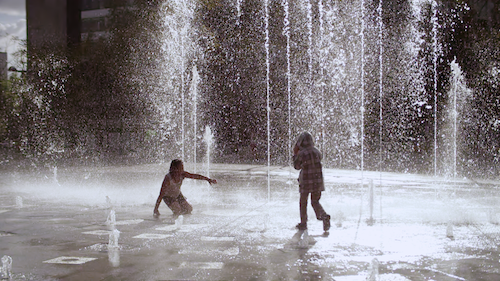
\includegraphics[width=\linewidth]{vignette-figs/elfuente_in.png}
  }
  \\
  \subfloat[Saliency map produced by MLNet~\cite{mlnet2016}, overlaid on input.]{
  \label{subfig:sal-still}
  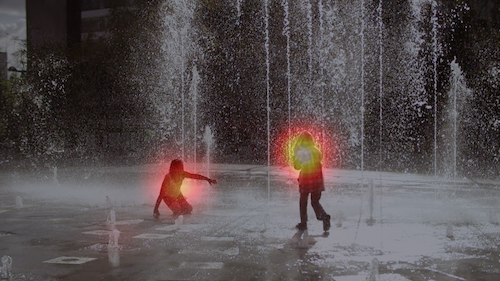
\includegraphics[width=\linewidth]{vignette-figs/elfuente_sal.png}
  }
  \\
  \subfloat[Perceptually-compressed \name video, 85\% smaller at iso-quality.]{
  \label{subfig:sal-vign}
  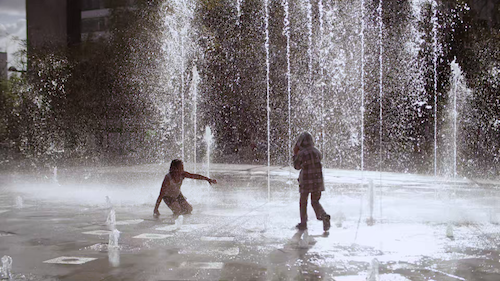
\includegraphics[width=\linewidth]{vignette-figs/elfuente_vignette.png}
  }
  \\
  \caption{Example video still, neural network-generated saliency map, and output \name perceptually compressed video.}
  \label{fig:example-vid-saliency}
\end{figure}


}


\newcommand{\systemOverviewFigure}{
\begin{figure*}[h]
% \begin{subfigure}{.48\textwidth}
%   \centering
%   \includegraphics[width=.9\linewidth]{vignette-figs/system-overview-open.pdf}
%   \caption{Open-loop offline saliency compression:~\name automatically generates saliency maps to include perceptual data during video transcoding.}
%   \label{fig:system-overview-open}
% \end{subfigure}\hfill%
% \begin{subfigure}{.48\textwidth}
%   \centering
%   \includegraphics[width=.9\linewidth]{vignette-figs/system-overview-closedloop.pdf}
%   \caption{Closed-loop re-compression:~\name~can leverage perceptual cues from VR headsets and other eyetracking devices to improve compression.}
%   \label{fig:sub2}
% \end{subfigure}
\caption{High-level architecture of~\name~system design.}

  \centering
  \subfloat[Open-loop offline saliency compression:~\name automatically generates saliency maps to include perceptual data during video transcoding.]{
    \label{fig:system-overview-open}
    \includegraphics[width=.46\textwidth]{system-overview-open.pdf}
  }
  \qquad
  \subfloat[Closed-loop re-compression:~\name~can leverage perceptual cues from VR headsets and other eyetracking devices to improve compression.]{
    \label{fig:system-overview-closed}
    \includegraphics[width=.46\textwidth]{system-overview-closedloop.pdf}
  }
  \caption{High-level architecture of~\name~system design.}
  \label{fig:system-overview}
\end{figure*}
}

\newcommand{\videoMetadataFigure}{
\begin{figure}
  \centering
  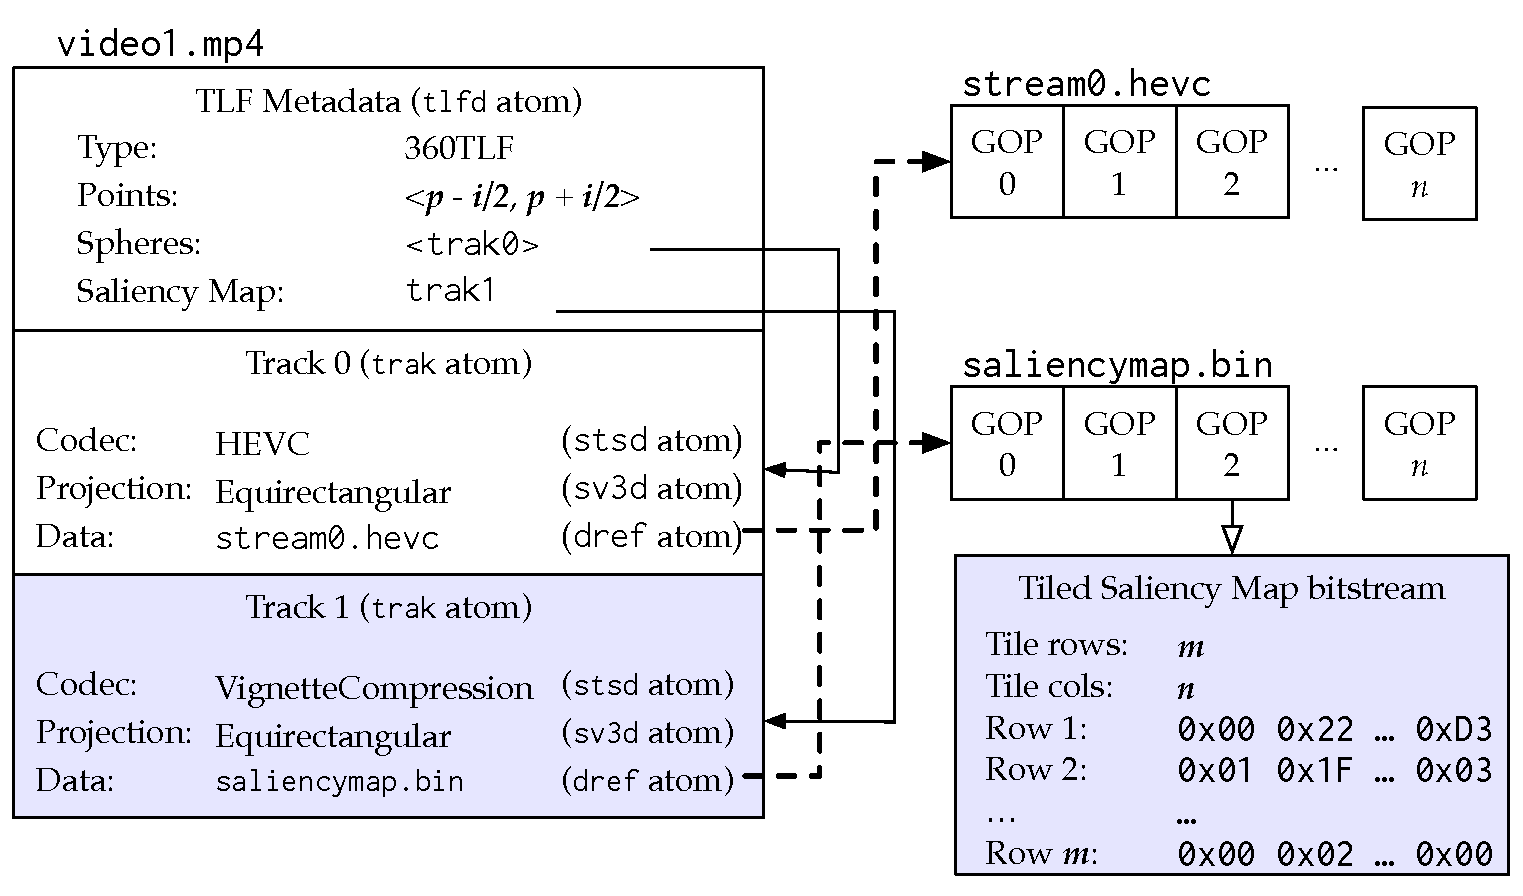
\includegraphics[width=\linewidth]{vignette-figs/physical-layout}
  \caption{Physical layout of video metadata in~\lightdb. \name-specific features are highlighted.}
  \label{fig:video-metadata}
\end{figure}
}

% \newcommand{\benchmarkInformationFigure}{
% \begin{figure}[t]
%   \centering
%    \subfloat[Benchmarks used for video profiling]{
%      	\label{table:benchmarks}
%        \resizebox{\linewidth}{!}{%
%        \begin{tabular}{l|l l l l}
%        Type                      & Benchmark & Description & Bitrate (Mbps) & Size (MB)        \\\hline
%        \multirow{2}{*}{Standard} & vbench~\cite{vbench}    & YouTube dataset & 0.53 - 470 & 757  \\
%                                  & Netflix~\cite{netflix2016data}   & Netflix dataset & 52 - 267 & 1123 \\
%        \multirow{2}{*}{VR}       & VR-360~\cite{saliency-map}    & 4K-360 dataset & 10 - 21 & 1400   \\
%                                  & Blender~\cite{blender}   & UHD / 3D movies & 10 - 147 & 6817 \\
%        \end{tabular}
%        }
%      } \\
%  \subfloat[Resolution and entropy distribution]{
%  \label{subfig:benchmark-entropy-res}
%   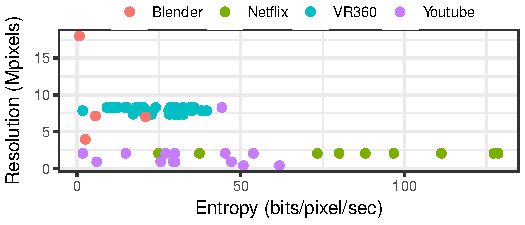
\includegraphics[width=\linewidth]{resolution-entropy2}
%
%  }
%   \caption{Characteristics of benchmark videos used to characterize \name. }
%   \label{fig:benchmark-info}
% \end{figure}
%
% }

\newcommand{\benchmarkInformationFigure}{
\begin{table}[h]
  \centering
       \begin{tabular}{l l l l l} \toprule
       Type                      & Benchmark & Description & Bitrate (Mbps) & Size (MB)        \\\midrule
       \multirow{2}{*}{Standard} & vbench~\cite{vbench}    & YouTube dataset & 0.53--470 & 757  \\
                                 & Netflix~\cite{netflix2016data}   & Netflix dataset & 52--267 & 1123 \\
       \multirow{2}{*}{VR}       & VR-360~\cite{saliency-map}    & 4K-360 dataset & 10--21 & 1400   \\
                                 & Blender~\cite{blender}   & UHD / 3D movies & 10--147 & 6817 \\ \bottomrule
       \end{tabular}


  \caption{Video datasets used to characterize \name. }
  \label{table:benchmarks}
\end{table}

}


\newcommand{\bitrateLadderFigure}{
\begin{figure}[h]
  \centering
  \subfloat[We varied bitrate and resolution for each video.]{
    \label{fig:bitrate-ladder-all}
    \includegraphics[width=1.05in]{vignette-figs/bitrate-ladders-subset}
  }
  \qquad
  \subfloat[The final bitrate ladder is the convex hull that maximizes PSNR.]{
    \label{fig:bitrate-ladder-max}
    \includegraphics[width=1.4in]{vignette-figs/bitrate-ladders-max}
  }

  \caption{Example bitrate ladder generated for one video in our dataset. We generated resolution-bitrate curves for all videos in our datasets.}

  \label{fig:bitrateladder}
\end{figure}

}

\newcommand{\avgStorageBitrateSavings}{
\begin{figure}
  \centering
    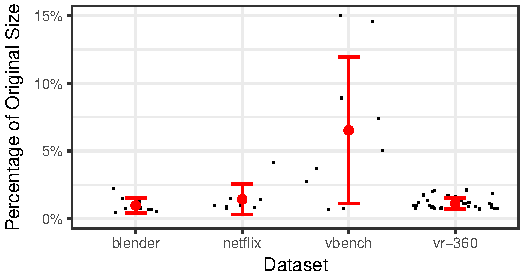
\includegraphics[width=\linewidth]{vignette-figs/bitrate-storage-savings}

  \caption{Aggregate storage savings by dataset. \nameCompress reduces videos to 1--15\% of their original size while maintaining PSNR of 34--39 dB and EWPSNR of 45-51 dB.}

  \label{fig:average-storage-bitrate-savings}
\end{figure}

}

\newcommand{\awsBreakevenFigure}{
\begin{figure}
  \centering
    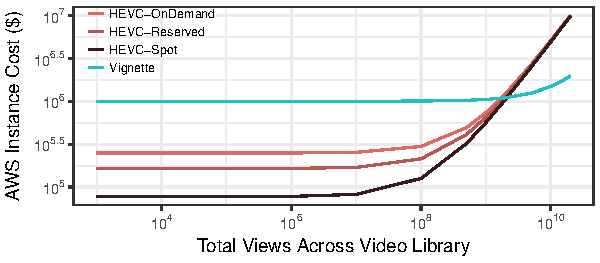
\includegraphics[width=\linewidth]{vignette-figs/aws-breakeven}
  \caption{Estimated AWS costs for deploying \name versus traditional video transcoding. \name's additional compute cost is amortized after $\scriptstyle\sim$2 billion video views over a 1-million video library.}

  \label{fig:aws-utilization}
\end{figure}

}
\newcommand{\powerFigure}{
\begin{figure}
  \centering
    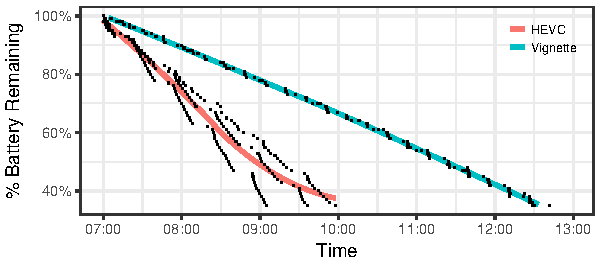
\includegraphics[width=\linewidth]{vignette-figs/power}
  \caption{Time to dissipate a Google Pixel 2 phone battery from 100\% to 30\% when viewing \hevc and \name videos continuously. \name videos provide 1.67$\times$ longer video playback on mobile phones.}

  \label{fig:power}
\end{figure}

}
